\documentclass{article}
\usepackage{graphicx}
\usepackage{hyperref}

\title{Playing Cards Object Detection Using YOLOv8}
\author{Teodor Kostadinov, student at \\Faculty of Mathematics and Informatics, Sofia University}
\date{}

\begin{document}

\maketitle

\begin{abstract}
This paper presents the development and evaluation of a machine learning model for detecting and identifying playing cards using the YOLOv8 architecture. The objective is to assist in card games by providing real-time card recognition. The study explores various approaches, including using synthetic and real datasets, augmentation techniques, and model fine-tuning.
\end{abstract}

\section{Introduction}
The goal is to develop an application capable of recognizing playing cards to assist in games like Blackjack, Bridge, Belot, and Poker. The project faced several challenges, including the lack of senior data science expertise and insufficient time to create a model from scratch or develop a comprehensive dataset.

\section{Methodology}

\subsection{Initial Approach}
To quickly implement the model, a pre-trained YOLOv8 model was chosen due to its accessibility through the Python Ultralytics library. However, the lack of a public dataset necessitated the use of a synthetic dataset.

\subsection{Datasets}
All playing cards datasets used during the training of the models are available in the project directory. All datasets are in YOLOv8 object detection format, split into \textit{train}, \textit{valid}, and \textit{test} directories with \textit{labels} and \textit{images} subdirectories. All datasets fall under the \href{https://creativecommons.org/publicdomain/zero/1.0/}{CC0: Public Domain} license.

\subsubsection{The Synthetic Dataset}
The synthetic dataset was copied from \href{https://www.kaggle.com/datasets/andy8744/playing-cards-object-detection-dataset}{Kaggle - Playing Cards Object Detection Dataset}. It includes 20,000 images synthetically generated and labeled with 52 classes. This dataset was used to train the YOLOv8m\_synthetic model.

\subsubsection{The "Real" Dataset}
The real dataset was created by the author, Teodor Kostadinov, and includes 100 images shot and labeled by the author using \href{https://labelstud.io/}{Label Studio} with 13 classes. This dataset was used to train the YOLOv8m\_real and YOLOv8m\_tuned models.

\subsubsection{The "Real" Augmented Dataset}
To address data scarcity, the real dataset was augmented using the \href{https://imgaug.readthedocs.io/en/latest/}{imgaug} library with the script \textit{augment\_dataset.ipynb}. This augmentation introduced 10 new augmented images for each image in the real dataset using various transformations, resulting in a total of 1,000 images. This augmented dataset was used to train the YOLOv8m\_aug model.

\subsubsection{The Combined Dataset}
The combined dataset was created using the \href{https://imgaug.readthedocs.io/en/latest/}{imgaug} library along with the scripts \textit{combine\_datasets.py} and \textit{transform\_labels\_in\_dataset.py}. It combines the full real dataset with 10 times more images taken from the synthetic dataset. This combined dataset was used to train the YOLOv8m\_comb model.

\subsection{Training Procedure}
The datasets were used to train various YOLOv8 models. The training was conducted using an NVIDIA RTX A2000 8GB GPU. The training details for each model are summarized in the following table:

\begin{table}[htbp]
\centering
\begin{tabular}{|c|c|c|c|}
\hline
\textbf{Model} & \textbf{Dataset} & \textbf{Epochs} & \textbf{Training Time} \\ \hline
YOLOv8m\_synthetic & 20,000 synthetic images & 10 & 2 hours \\ \hline
YOLOv8m\_real & 100 real images & 100 & 20 minutes \\ \hline
YOLOv8m\_aug & 1,000 augmented images & 100 & 40 minutes \\ \hline
YOLOv8m\_comb & 100 real + 1,000 synthetic & 100 & 50 minutes \\ \hline
YOLOv8m\_tuned & 100 real images & 100 & 10 minutes \\ \hline
\end{tabular}
\caption{Training details for YOLOv8 models}
\label{table:1}
\end{table}

\newpage
\section{Results}

\subsection{YOLOv8\_Synthetic Model}
\begin{itemize}
  \item \textbf{Training:} 20,000 images, 10 epochs, NVIDIA RTX A2000 8GB
  \item \textbf{Performance:} ~99\% accuracy on the test set
\end{itemize}

\begin{figure}[htbp]
  \centering
  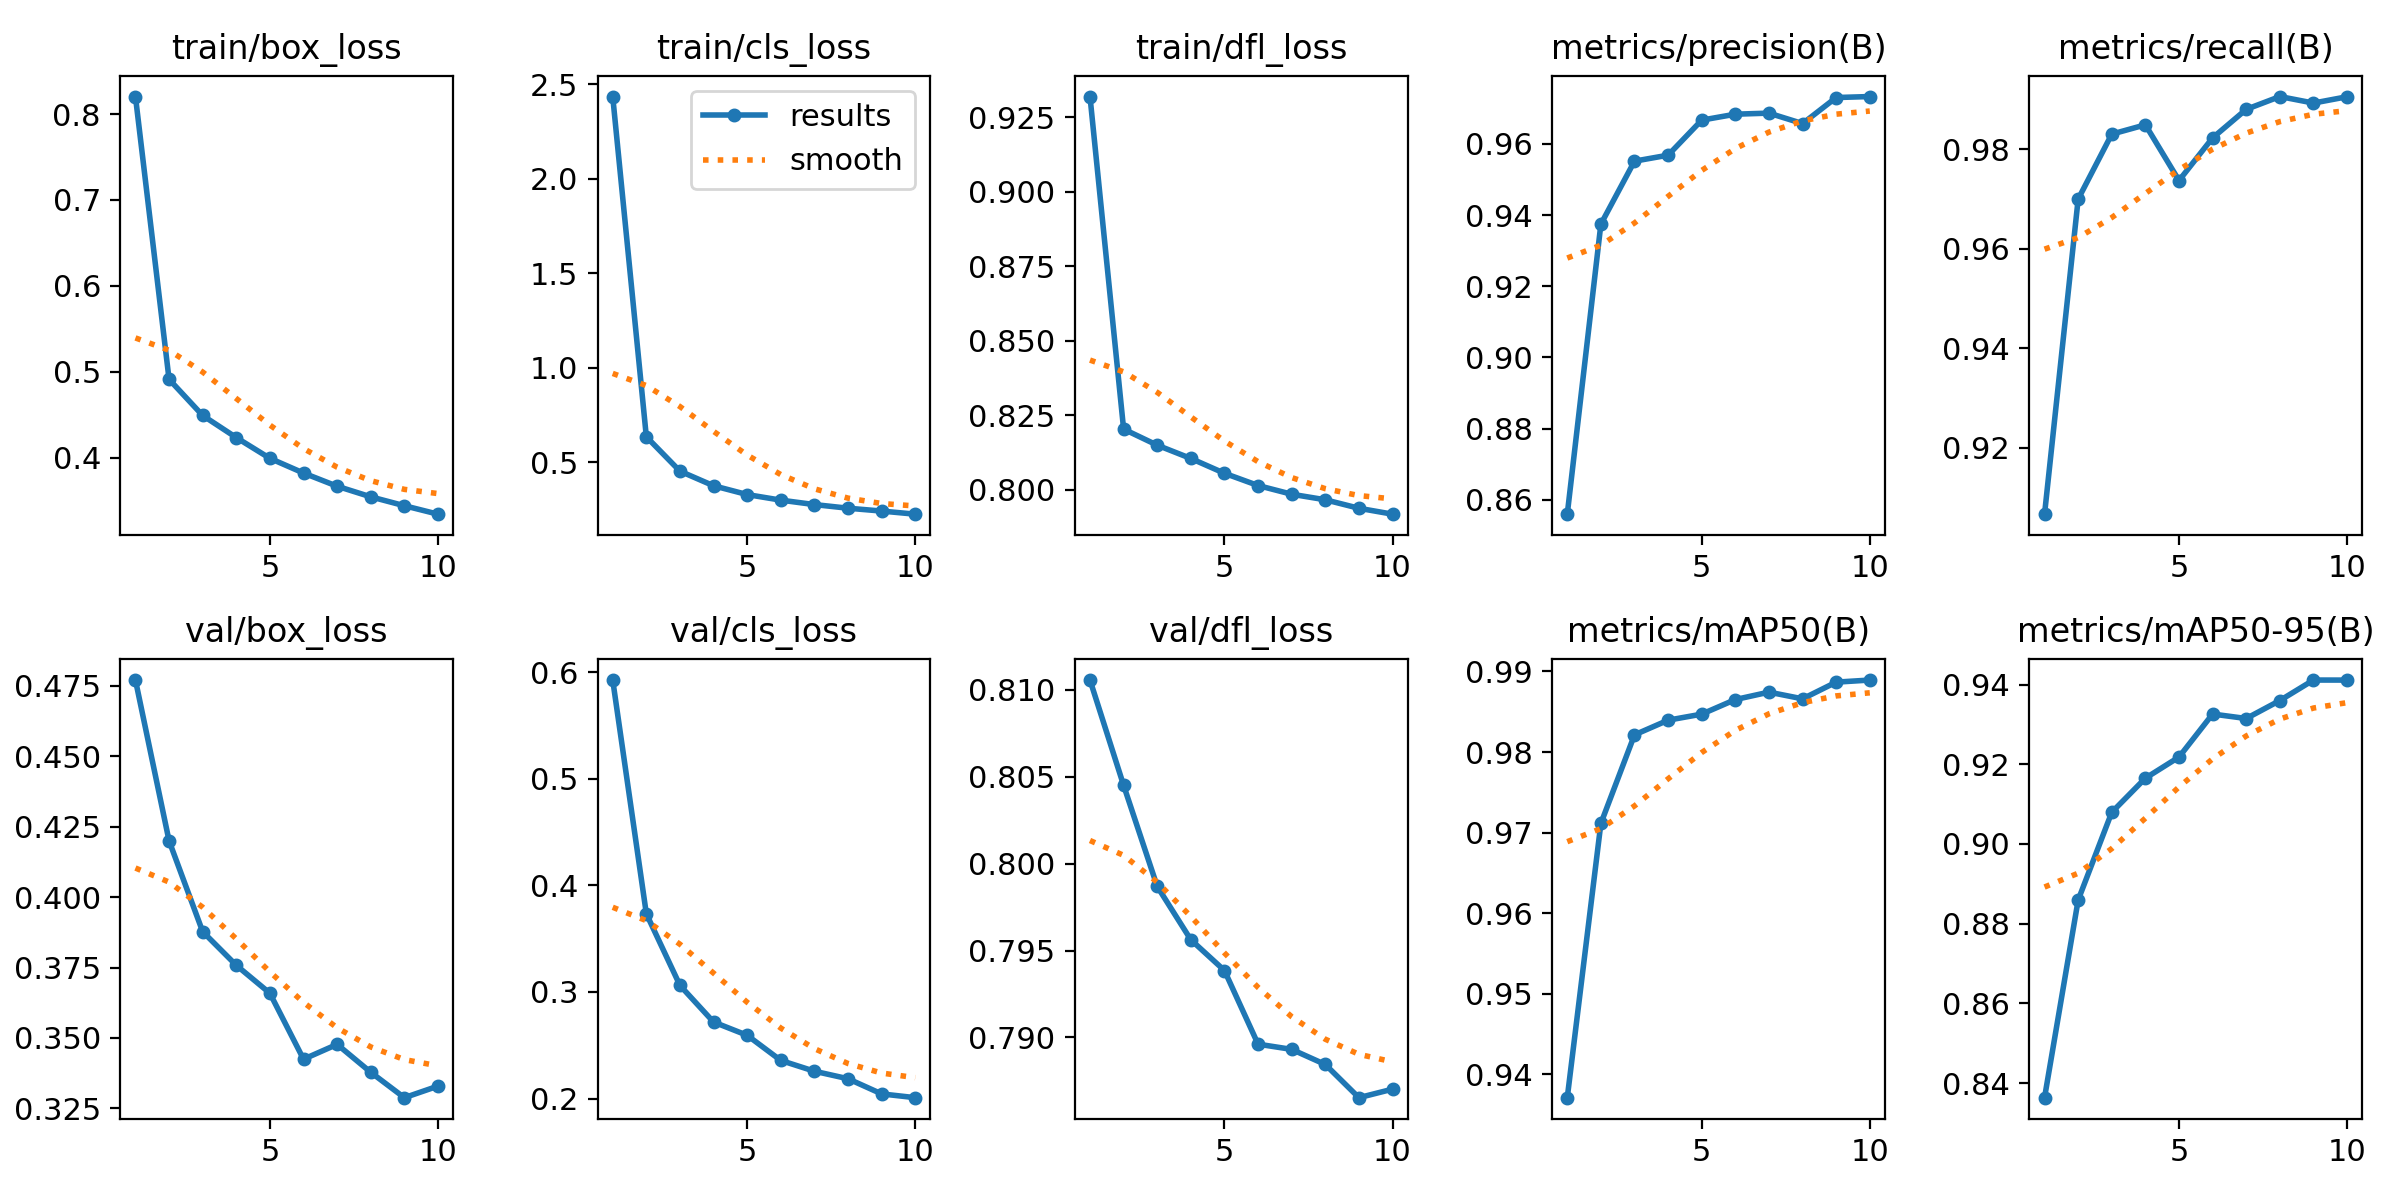
\includegraphics[width=0.8\textwidth]{./media/yolov8_synthetic_results.png}
  \caption{YOLOv8\_Synthetic Model Results}
  \label{fig:synthetic_results}
\end{figure}

\subsection{YOLOv8\_Real Model}
\begin{itemize}
  \item \textbf{Training:} 100 images, 100 epochs, NVIDIA RTX A2000 8GB
  \item \textbf{Performance:} Limited due to the small dataset
\end{itemize}
\begin{figure}[htbp]
  \centering
  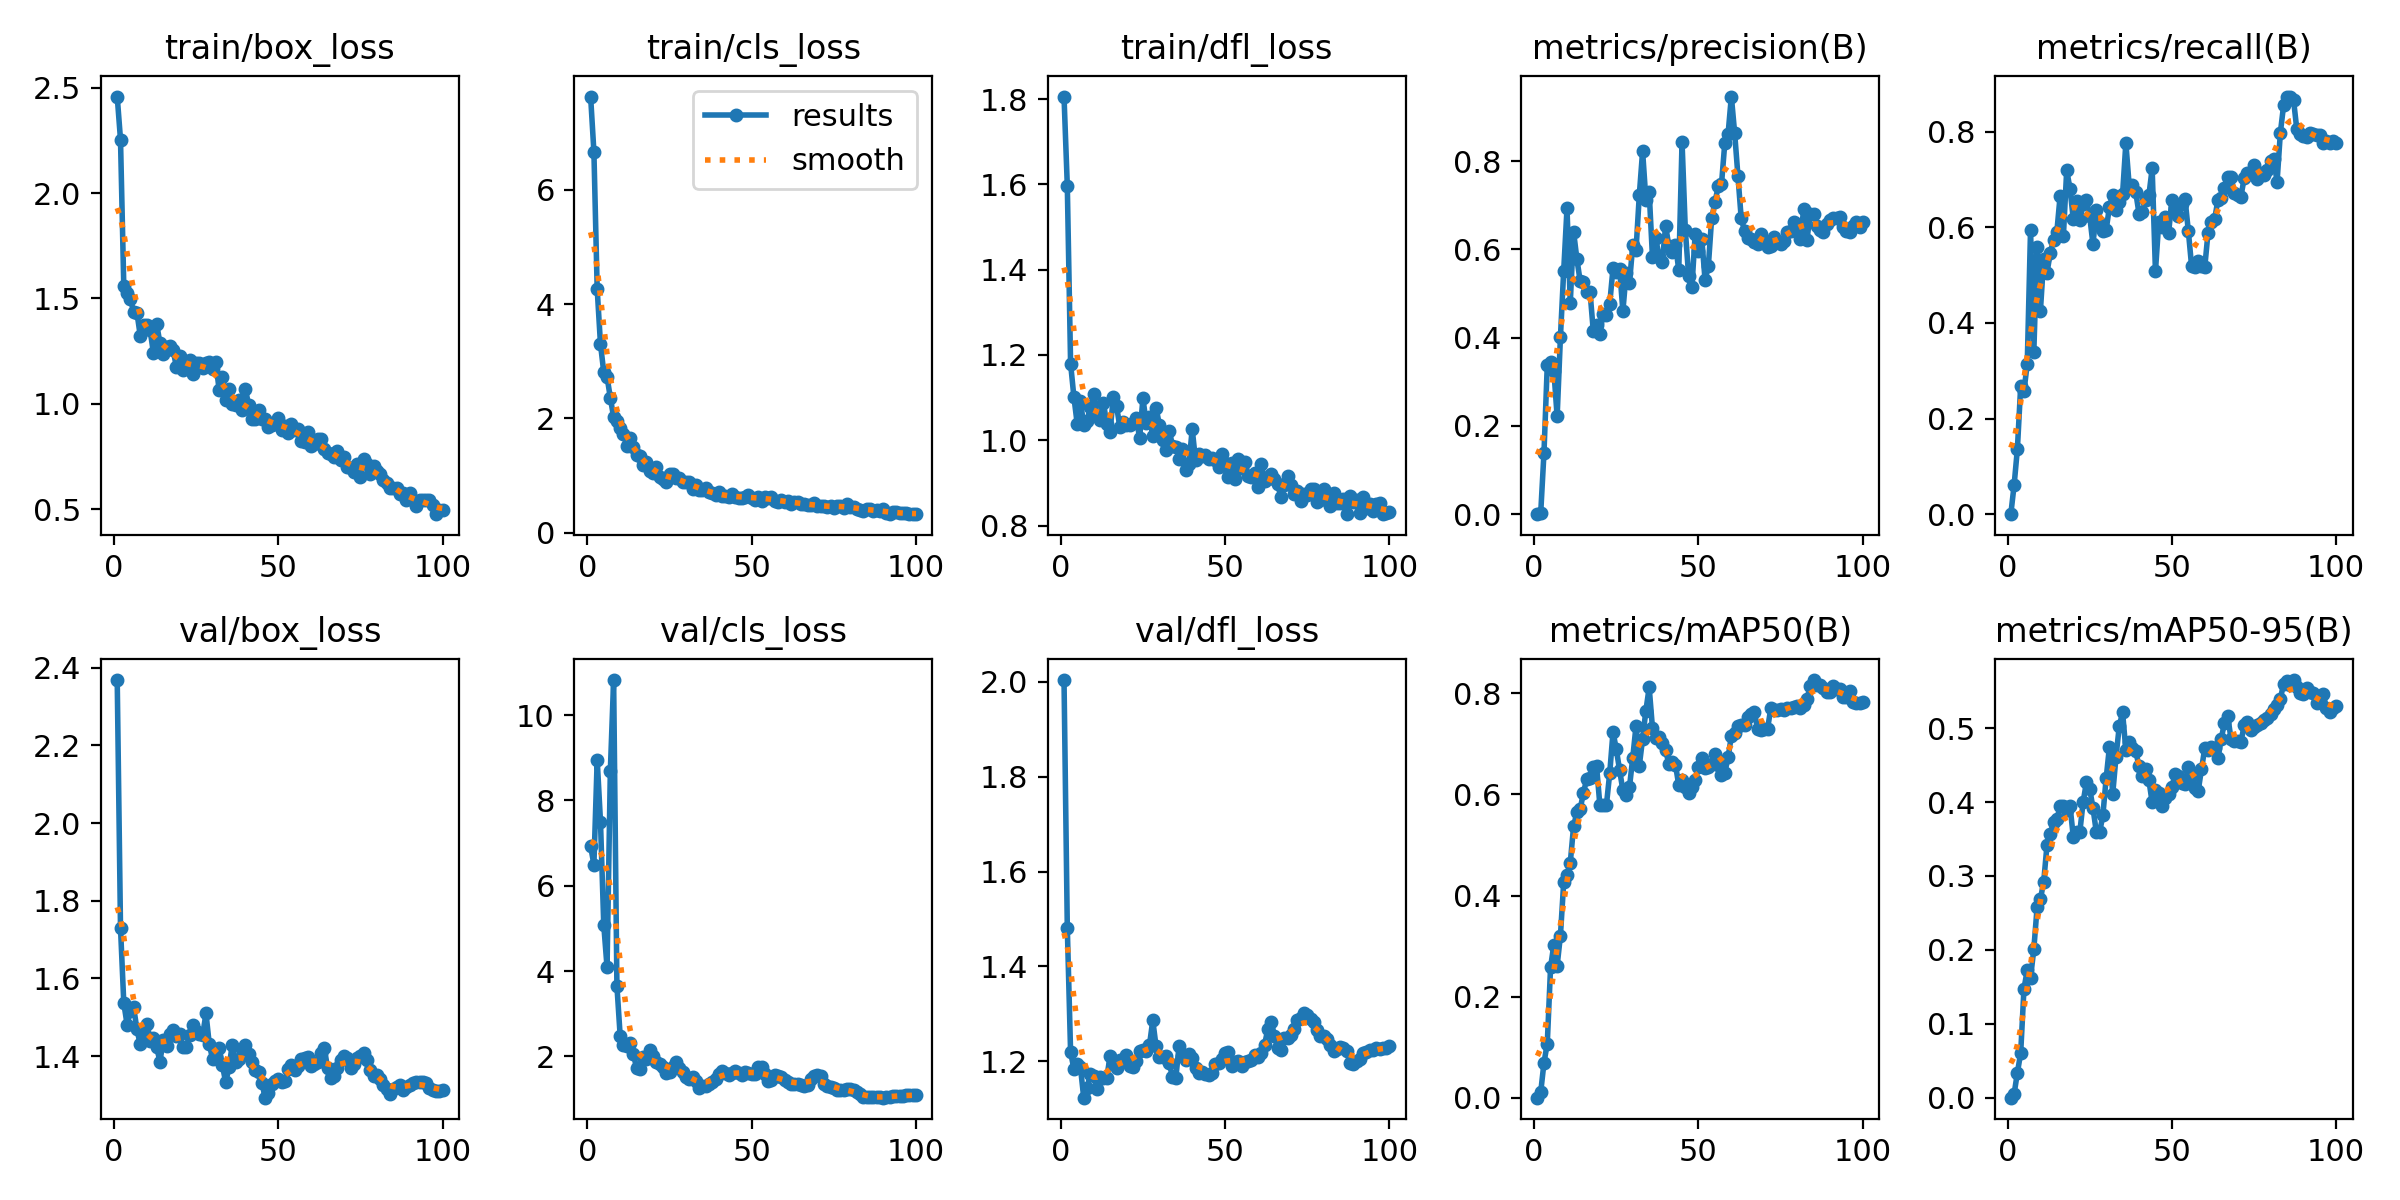
\includegraphics[width=0.8\textwidth]{./media/yolov8_real_results.png}
  \caption{YOLOv8\_Real Model Results}
  \label{fig:real_results}
\end{figure}

\subsection{YOLOv8\_Augmented Model}
\begin{itemize}
  \item \textbf{Training:} 1,000 images, 100 epochs, NVIDIA RTX A2000 8GB
  \item \textbf{Performance:} Similar to YOLOv8\_Real
\end{itemize}

\begin{figure}[htbp]
  \centering
  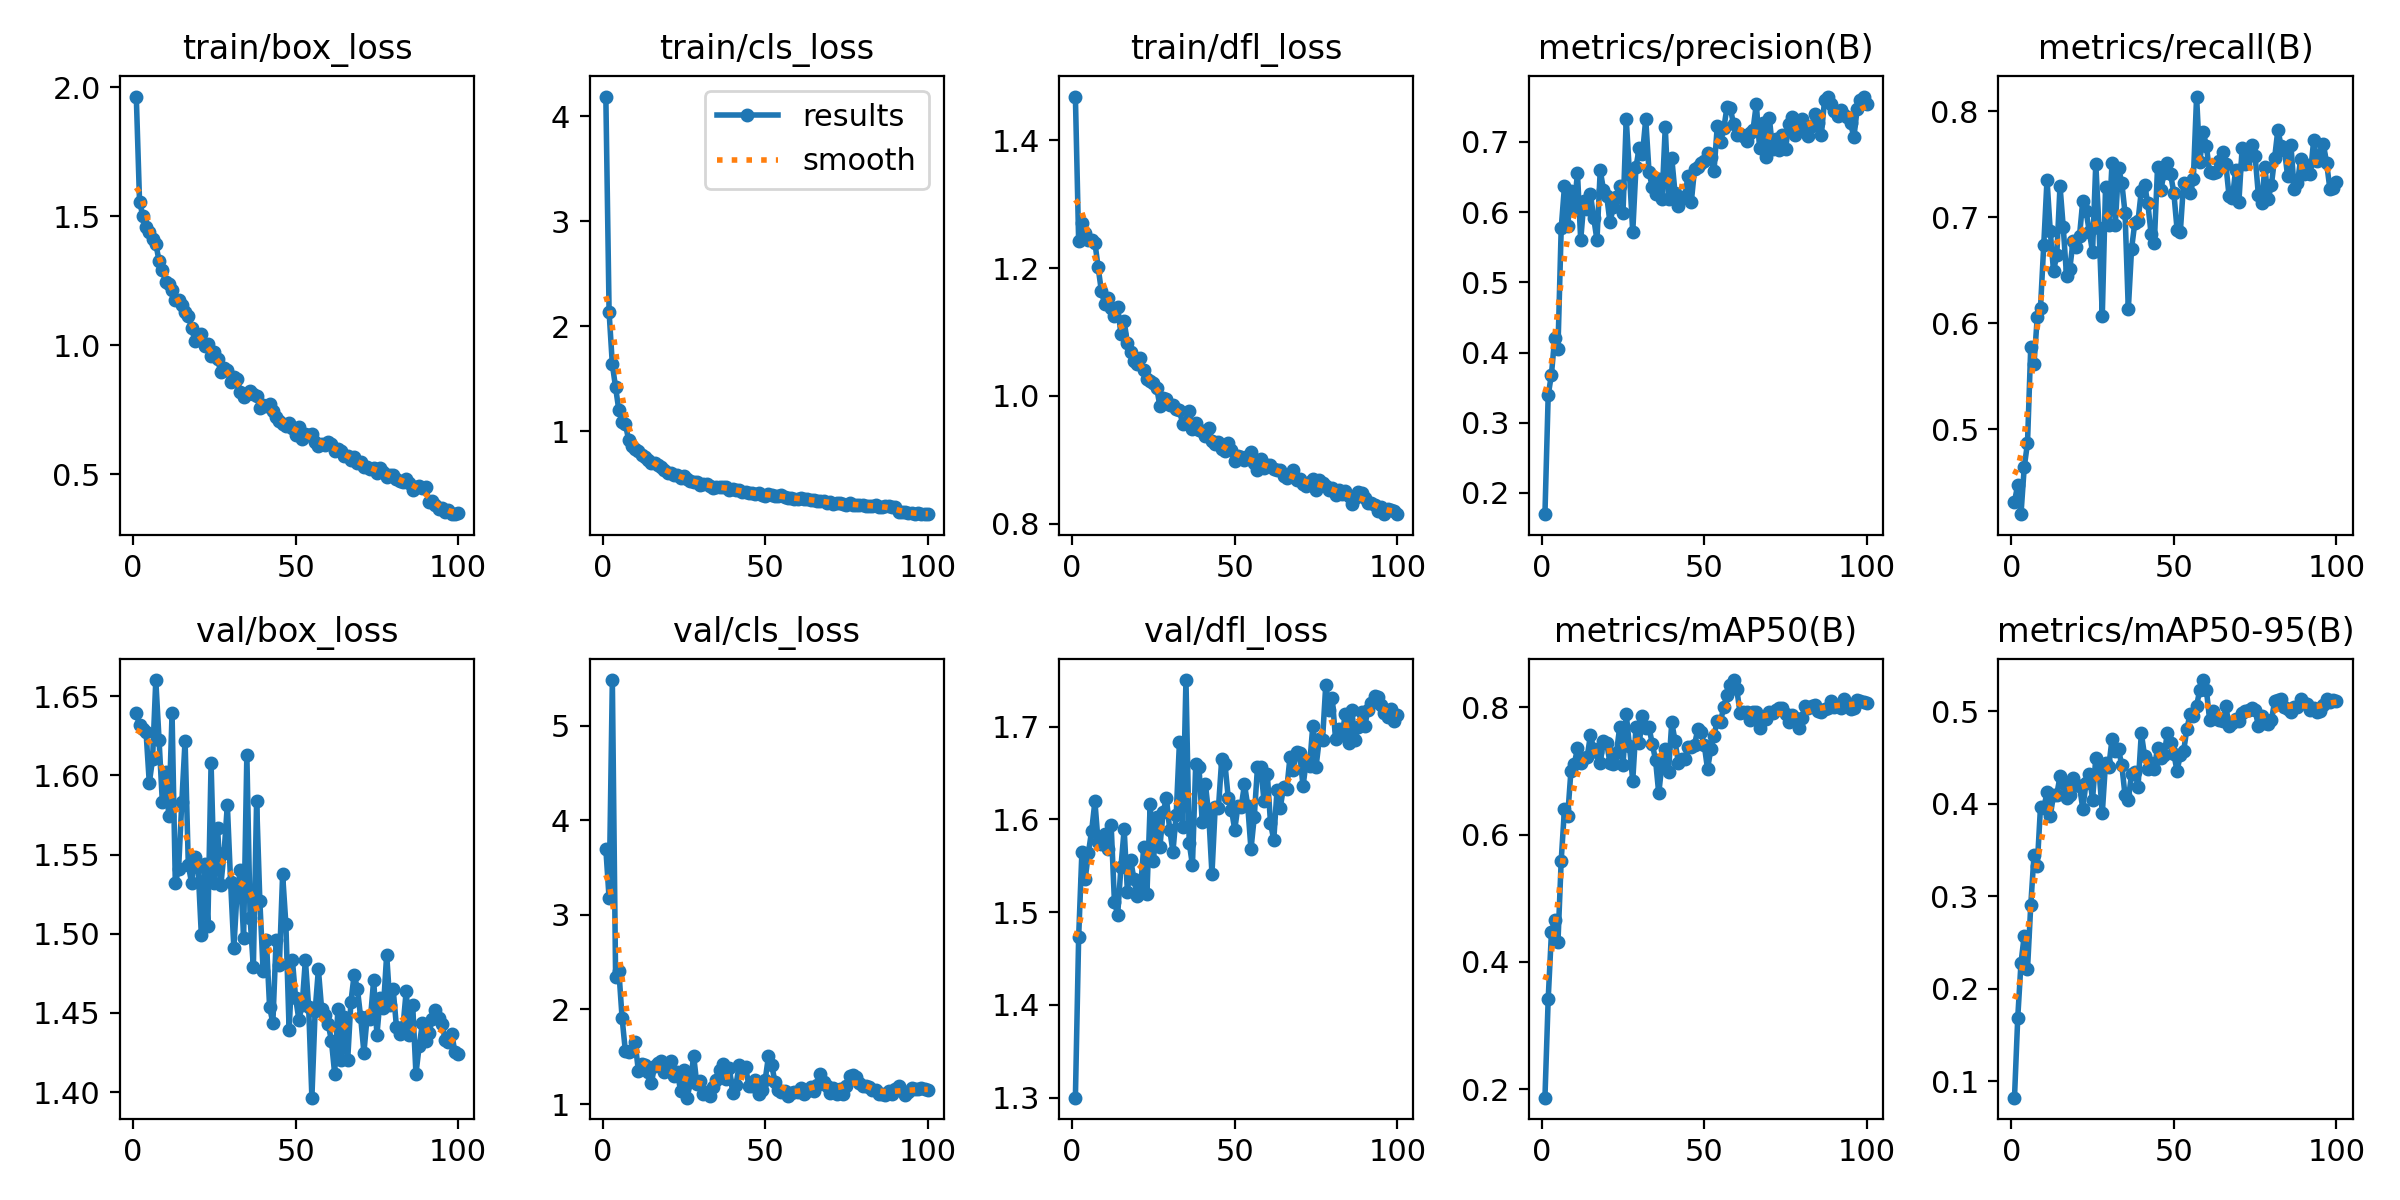
\includegraphics[width=0.8\textwidth]{./media/yolov8_aug_results.png}
  \caption{YOLOv8\_Augmented Model Results}
  \label{fig:augmented_results}
\end{figure}

\subsection{YOLOv8\_Combined Model}
\begin{itemize}
  \item \textbf{Training:} 1,100 images, 100 epochs, NVIDIA RTX A2000 8GB
  \item \textbf{Performance:} Worse than synthetic-only model
\end{itemize}
\begin{figure}[htbp]
  \centering
  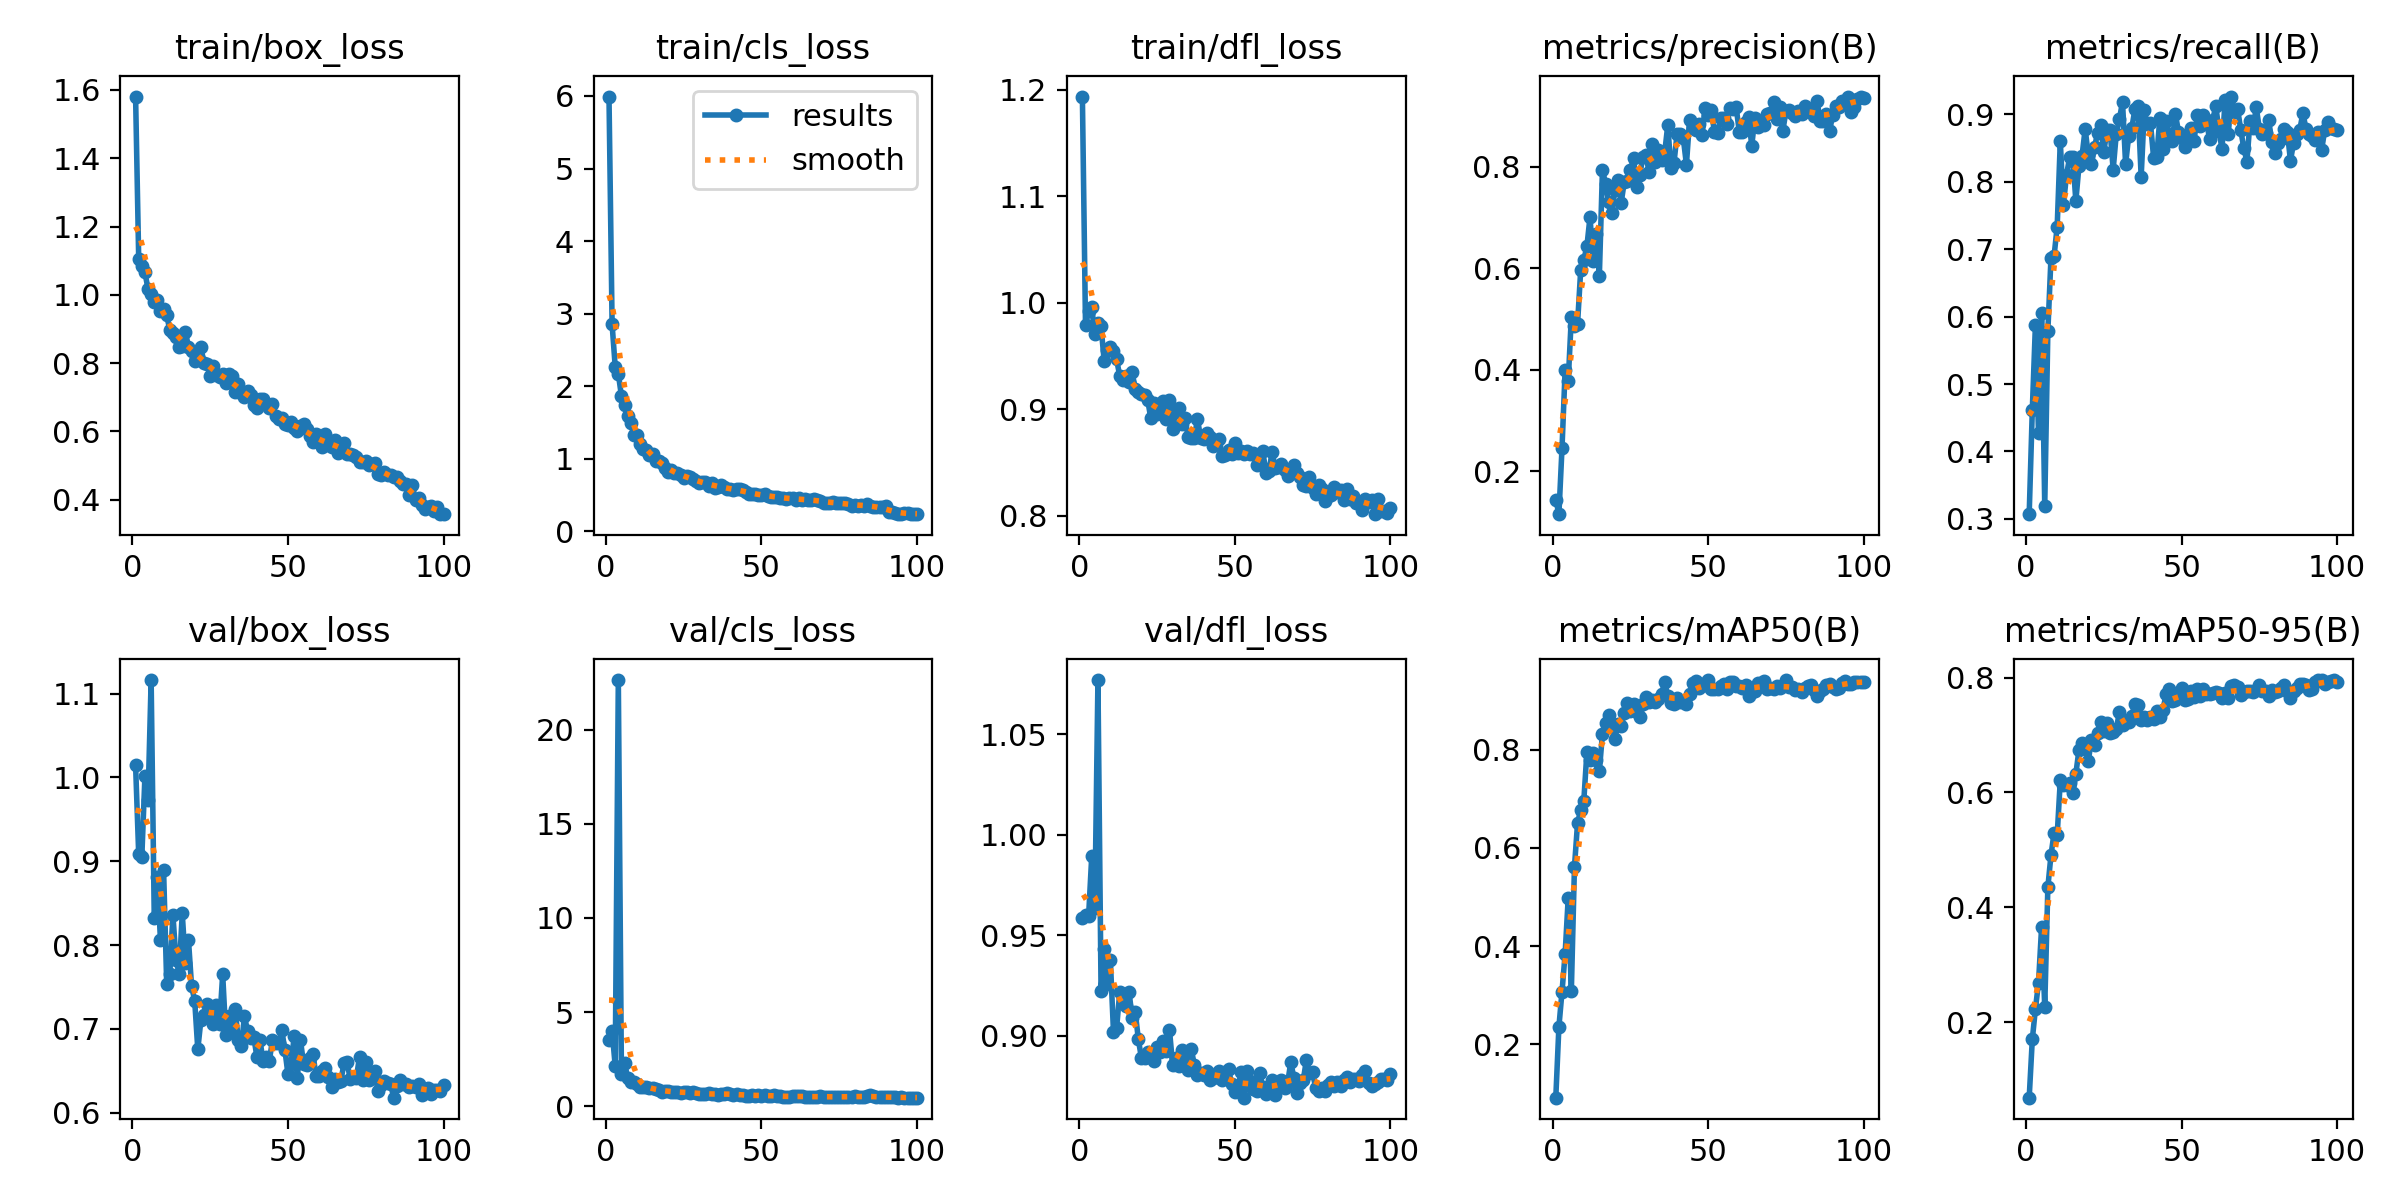
\includegraphics[width=0.8\textwidth]{./media/yolov8_comb_results.png}
  \caption{YOLOv8\_Combined Model Results}
  \label{fig:combined_results}
\end{figure}

\newpage
\subsection{YOLOv8\_Tuned Model}
\begin{itemize}
  \item \textbf{Training:} Fine-tuned with 100 real images
  \item \textbf{Performance:} Improved detection of specific cards like Ace of Hearts but issues with suit differentiation
\end{itemize}
\begin{figure}[htbp]
  \centering
  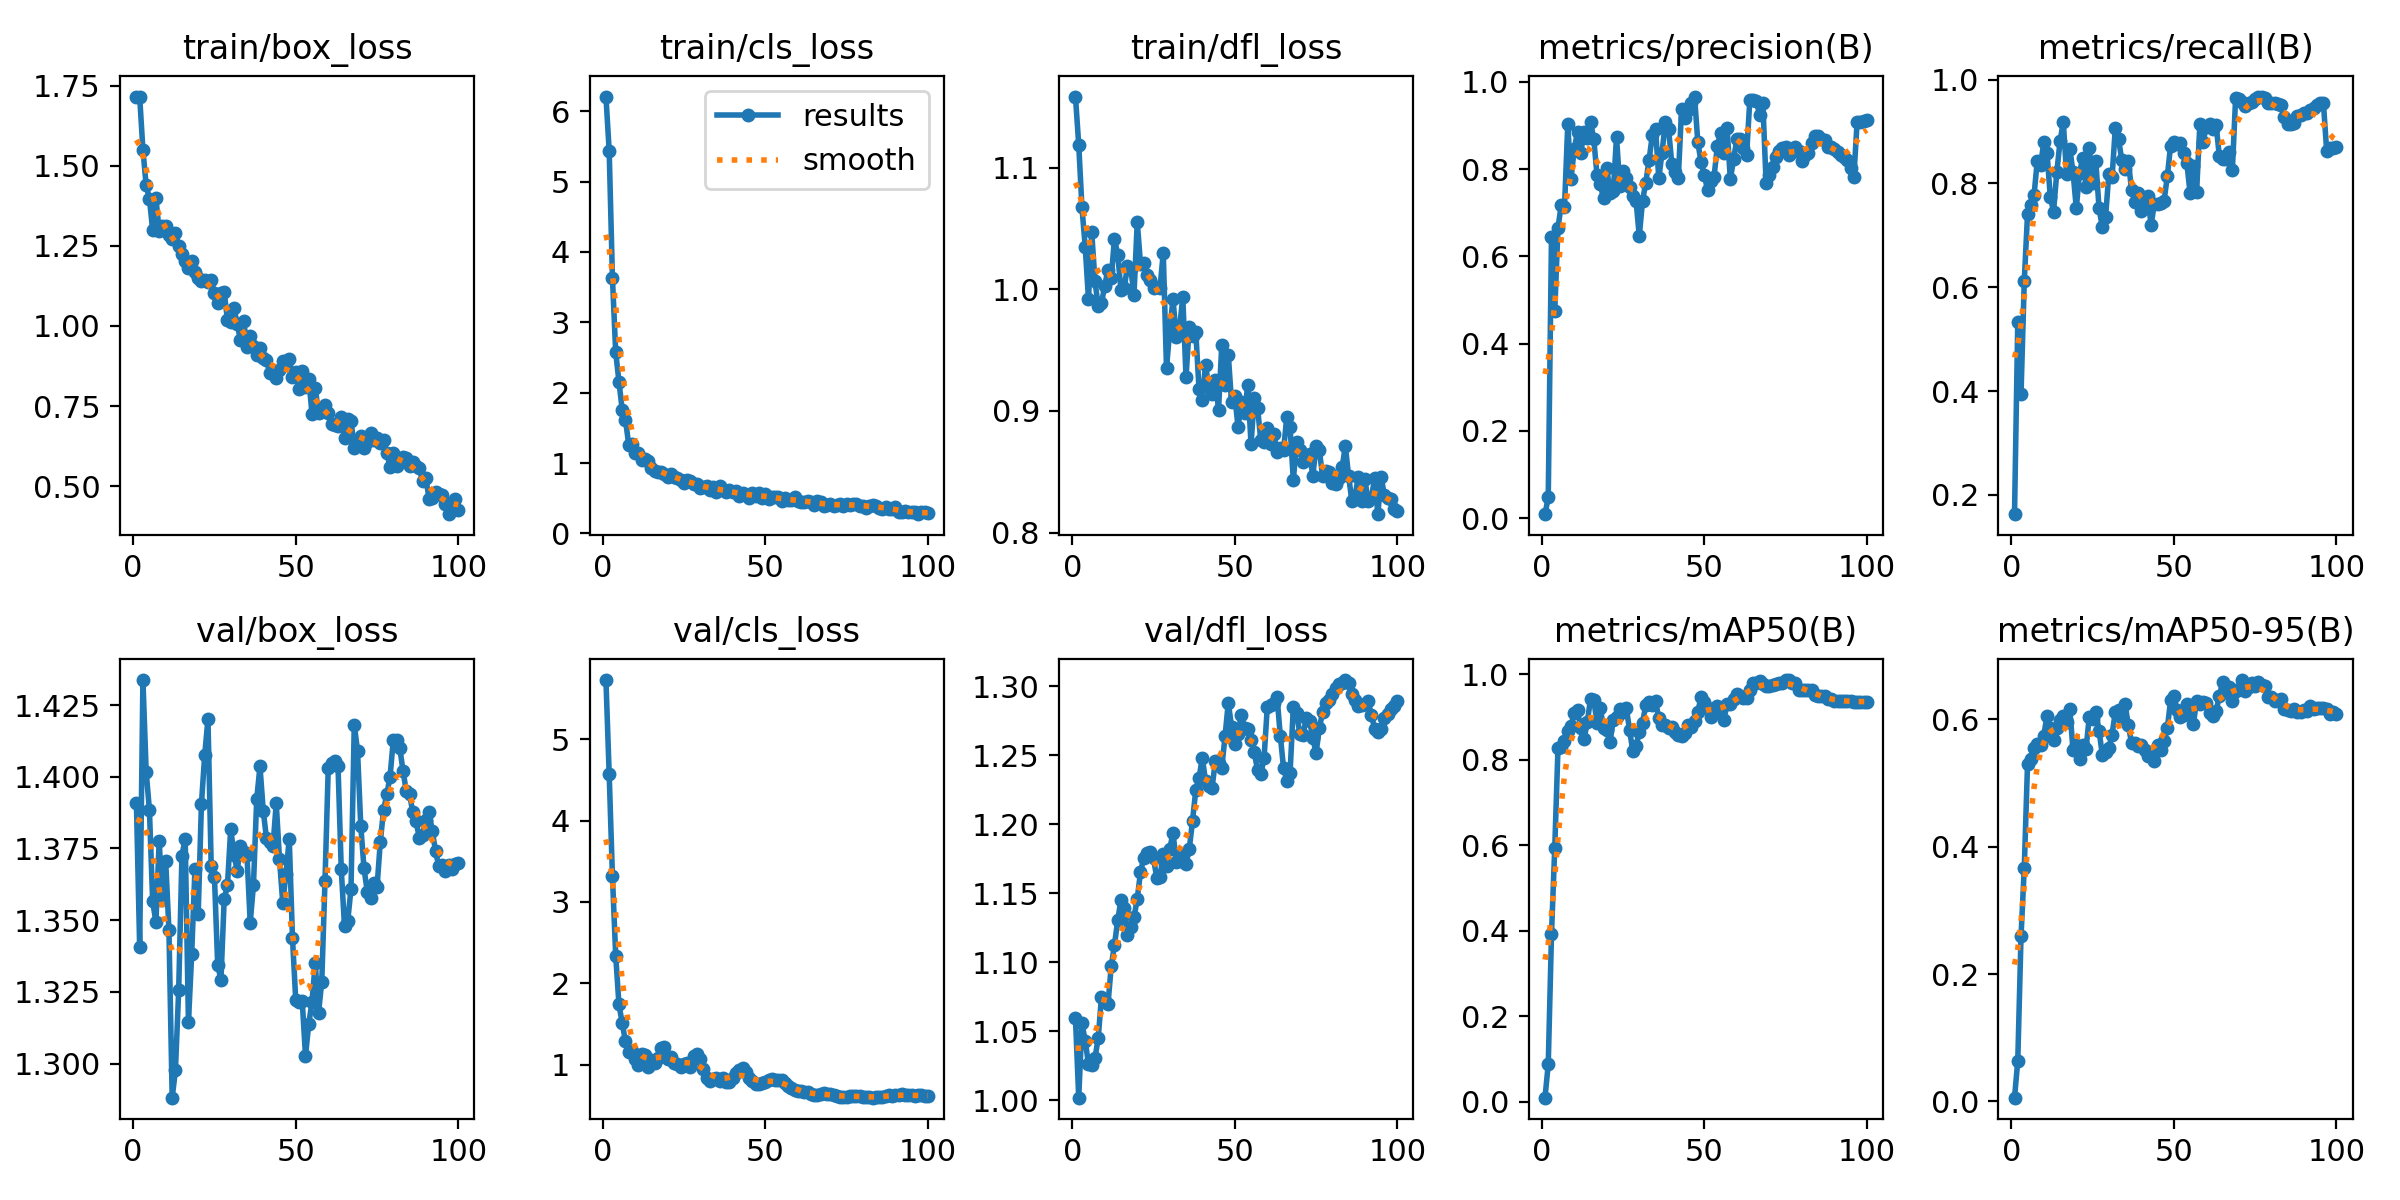
\includegraphics[width=0.8\textwidth]{./media/yolov8_tuned_results.png}
  \caption{YOLOv8\_Tuned Model Results}
  \label{fig:tuned_results}
\end{figure}


\section{Discussion}
The study demonstrates that using a synthetic dataset with YOLOv8 can yield high accuracy for card detection under controlled conditions. Real-life datasets require more data to achieve comparable results. Augmentation alone did not significantly improve performance. Fine-tuning synthetic models with real data shows promise, but further refinement and more data are necessary.

\section{Conclusion}
More data generally leads to better results in object detection tasks. Fine-tuning synthetic models with real-life data appears to be a viable strategy, though combining datasets effectively remains challenging. Future work should focus on increasing the dataset size and exploring better data augmentation and combination techniques.

\section{References}
\begin{itemize}
  \item \href{https://www.kaggle.com/datasets/andy8744/playing-cards-object-detection-dataset}{Playing Cards Object Detection Dataset on Kaggle}
  \item \href{https://www.robots.ox.ac.uk/~vgg/data/dtd/}{DTD Dataset}
  \item \href{https://imgaug.readthedocs.io/en/latest/}{imgaug Documentation}
\end{itemize}

\end{document}
